%% LyX 2.1.0 created this file.  For more info, see http://www.lyx.org/.
%% Do not edit unless you really know what you are doing.
\documentclass[11pt,oneside,english]{book}
\usepackage[T1]{fontenc}
\usepackage[latin9]{inputenc}
\usepackage{geometry}
\geometry{verbose,tmargin=3cm,bmargin=3cm,lmargin=2.5cm,rmargin=2.5cm}
\setcounter{secnumdepth}{3}
\setcounter{tocdepth}{3}
\usepackage{amsthm}
\usepackage{amsmath}
\usepackage{graphicx}
\usepackage{esint}


\makeatletter
%%%%%%%%%%%%%%%%%%%%%%%%%%%%%% Textclass specific LaTeX commands.
\numberwithin{equation}{section}
\numberwithin{figure}{section}

%%%%%%%%%%%%%%%%%%%%%%%%%%%%%% User specified LaTeX commands.
\IfFileExists{lmodern.sty}{\usepackage{lmodern}}{}

\makeatother

\usepackage{babel}
\begin{document}

\title{\textbf{3D-Parabolised Stability Equations}}


\author{Anil Kumar Singh}

\maketitle

\chapter{Parabolized Stability Equations}

Incompressible fluid flow is governed by mass conservation (continuity
equation) and momentum equations (Navier-stokes equations) which are
written below%
\footnote{{*} marked quantities are dimensional%
}.

Continuity Equation

\[
\frac{\partial u^{*}}{\partial x^{*}}+\frac{\partial v^{*}}{\partial y^{*}}+\frac{\partial w^{*}}{\partial z^{*}}=0
\]


and Navier Stokes equations

\[
\rho\left[\frac{\partial u^{*}}{\partial t^{*}}+u^{*}\frac{\partial u^{*}}{\partial x^{*}}+v^{*}\frac{\partial u^{*}}{\partial y^{*}}+w^{*}\frac{\partial u^{*}}{\partial z^{*}}\right]=-\frac{\partial p^{*}}{\partial x^{*}}+\mu\left[\frac{\partial^{2}}{\partial x^{*2}}+\frac{\partial^{2}}{\partial y^{*2}}+\frac{\partial^{2}}{\partial z^{*2}}\right]u^{*}
\]


\[
\rho\left[\frac{\partial v^{*}}{\partial t^{*}}+u^{*}\frac{\partial v^{*}}{\partial x^{*}}+v^{*}\frac{\partial v^{*}}{\partial y^{*}}+w^{*}\frac{\partial v^{*}}{\partial z^{*}}\right]=-\frac{\partial p^{*}}{\partial y^{*}}+\mu\left[\frac{\partial^{2}}{\partial x^{*2}}+\frac{\partial^{2}}{\partial y^{*2}}+\frac{\partial^{2}}{\partial z^{*2}}\right]v^{*}
\]


\[
\rho\left[\frac{\partial w^{*}}{\partial t^{*}}+u^{*}\frac{\partial w^{*}}{\partial x^{*}}+v^{*}\frac{\partial w^{*}}{\partial y^{*}}+w^{*}\frac{\partial w^{*}}{\partial z^{*}}\right]=-\frac{\partial p^{*}}{\partial z^{*}}+\mu\left[\frac{\partial^{2}}{\partial x^{*2}}+\frac{\partial^{2}}{\partial y^{*2}}+\frac{\partial^{2}}{\partial z^{*2}}\right]w^{*}
\]


Non-dimensional form of these equations can be obtained by specifying
non dimensional quantities as shown below

\[
x=\frac{x^{*}}{L},\quad y=\frac{y^{*}}{L},\quad z=\frac{z^{*}}{L},
\]


\[
u=\frac{u^{*}}{U},\quad v=\frac{v^{*}}{U},\quad w=\frac{w^{*}}{U},
\]


\[
t=\frac{Ut^{*}}{L},\quad p=\frac{p^{*}}{\rho U^{2}},\quad Re=\frac{\rho UL}{\mu},
\]


Substituting in above continuity and momentum equations we get non-dimensional
equations 

\[
\frac{\partial u}{\partial x}+\frac{\partial v}{\partial y}+\frac{\partial w}{\partial z}=0
\]


\[
\frac{\partial u}{\partial t}+u\frac{\partial u}{\partial x}+v\frac{\partial u}{\partial y}+w\frac{\partial u}{\partial z}=-\frac{\partial p}{\partial x}+\frac{1}{Re}\left[\frac{\partial^{2}u}{\partial x^{2}}+\frac{\partial^{2}u}{\partial y^{2}}+\frac{\partial^{2}u}{\partial z^{2}}\right]
\]


\[
\frac{\partial v}{\partial t}+u\frac{\partial v}{\partial x}+v\frac{\partial v}{\partial y}+w\frac{\partial v}{\partial z}=-\frac{\partial p}{\partial y}+\frac{1}{Re}\left[\frac{\partial^{2}v}{\partial x^{2}}+\frac{\partial^{2}v}{\partial y^{2}}+\frac{\partial^{2}v}{\partial z^{2}}\right]
\]


\[
\frac{\partial w}{\partial t}+u\frac{\partial w}{\partial x}+v\frac{\partial w}{\partial y}+w\frac{\partial w}{\partial z}=-\frac{\partial p}{\partial z}+\frac{1}{Re}\left[\frac{\partial^{2}w}{\partial x^{2}}+\frac{\partial^{2}w}{\partial y^{2}}+\frac{\partial^{2}w}{\partial z^{2}}\right]
\]



\section{Linearized Stability Equations}

Let

\[
q(x,y,z,t)=\bar{q}(x,y,z)+q'(x,y,z,t)
\]


Above equations are satisfied by instantaneous quantities $q(x,y,z,t)$
and base flow $\bar{q}(x,y,z,t)$. Writing continuity and momentum
for both and subtracting one from other give following linearized
stability equations.

\[
\frac{\partial u'}{\partial x}+\frac{\partial v'}{\partial y}+\frac{\partial w'}{\partial z}=0
\]


\[
\frac{\partial u'}{\partial t}+u'\frac{\partial\bar{u}}{\partial x}+v'\frac{\partial\bar{u}}{\partial y}+w'\frac{\partial\bar{u}}{\partial z}+\bar{u}\frac{\partial u'}{\partial x}+\bar{v}\frac{\partial u'}{\partial y}+\bar{w}\frac{\partial u'}{\partial z}=-\frac{\partial p'}{\partial x}+\frac{1}{Re}\left[\frac{\partial^{2}u'}{\partial x^{2}}+\frac{\partial^{2}u'}{\partial y^{2}}+\frac{\partial^{2}u'}{\partial z^{2}}\right]
\]


\[
\frac{\partial v'}{\partial t}+u'\frac{\partial\bar{v}}{\partial x}+v'\frac{\partial\bar{v}}{\partial y}+w'\frac{\partial\bar{v}}{\partial z}+\bar{u}\frac{\partial v'}{\partial x}+\bar{v}\frac{\partial v'}{\partial y}+\bar{w}\frac{\partial v'}{\partial z}=-\frac{\partial p'}{\partial y}+\frac{1}{Re}\left[\frac{\partial^{2}v'}{\partial x^{2}}+\frac{\partial^{2}v'}{\partial y^{2}}+\frac{\partial^{2}v'}{\partial z^{2}}\right]
\]


\[
\frac{\partial w'}{\partial t}+u'\frac{\partial\bar{w}}{\partial x}+v'\frac{\partial\bar{w}}{\partial y}+w'\frac{\partial\bar{w}}{\partial z}+\bar{u}\frac{\partial w'}{\partial x}+\bar{v}\frac{\partial w'}{\partial y}+\bar{w}\frac{\partial w'}{\partial z}=-\frac{\partial p'}{\partial z}+\frac{1}{Re}\left[\frac{\partial^{2}w'}{\partial x^{2}}+\frac{\partial^{2}w'}{\partial y^{2}}+\frac{\partial^{2}w'}{\partial z^{2}}\right]
\]


where 

\[
q'(x,y,z,t)=\tilde{q}(x,y,z)\exp i\Theta
\]



\section{Parabolized Stability Equations}

For different analysis type $\tilde{q}$ and $\Theta$ take different
form. For example, for a bi-global analysis $\tilde{q}(x,y,z)=\tilde{q}(x,y)$
and $\Theta=\beta z-\omega t$ . For Orr-sommerfeld equations $\tilde{q}(x,y,z)=\tilde{q}(y)$
and $\Theta=\alpha x+\beta z-\omega t$ .The introduction of a harmonic
decomposition in $x$ and $z$ implies homogeneity of the base flow
in these directions. These conditions, however, are too restrictive
for complicated vortical flows and those around two-dimensional bodies.
Consequently, the flow is assumed to be general in a two-dimensional
plane, and mildly inhomogeneous in the third direction which is permitted
by allowing the axial wavenumber to vary slowly. This leads to the
parabolised stability equation concept, formally introduced by Herbert\cite{key-1}.

\[
q'(x,y,z,t)=\tilde{q}(x,y,z)\exp i\Theta
\]


where $\Theta=\intop_{z_{0}}^{z}\beta(\xi)d\xi-\omega t$

\[
\frac{\partial q'}{\partial z}=\left\{ i\beta\tilde{q}+\frac{\partial\tilde{q}}{\partial z}\right\} \exp i\Theta
\]


and

\[
\frac{\partial^{2}q'}{\partial z^{2}}=\left\{ \frac{\partial^{2}\tilde{q}}{\partial z^{2}}+2i\beta\frac{\partial\tilde{q}}{\partial z}-\beta^{2}\tilde{q}+i\frac{d\beta}{dz}\tilde{q}\right\} \exp i\Theta
\]


$\beta$ is streamwise wavenumber complex in nature given as $\beta(\xi)=$$\beta_{r}(\xi)+i\beta_{i}(\xi)$. 

It should be noted that $\tilde{q}(x,y,z)$ depends very weakly on
$z$ coordinate hence, second derivatives w.r.t $z$ will be neglected.
Therefore,

\[
\frac{\partial^{2}q'}{\partial z^{2}}\approx\left\{ 2i\beta\frac{\partial\tilde{q}}{\partial z}-\beta^{2}\tilde{q}+i\frac{d\beta}{dz}\tilde{q}\right\} \exp i\Theta
\]


Above form of perturbations if fetched in linearized stability equations
to derive PSE as shown below.

Continuity equation

\begin{equation}
\frac{\partial\tilde{u}}{\partial x}+\frac{\partial\tilde{v}}{\partial y}+\frac{\partial\tilde{w}}{\partial z}+i\beta\tilde{w}=0
\end{equation}


$x$ momentum equation

\[
-i\omega\tilde{u}+\frac{\partial\bar{u}}{\partial x}\tilde{u}+\frac{\partial\bar{u}}{\partial y}\tilde{v}+\frac{\partial\bar{u}}{\partial z}\tilde{w}+\bar{u}\frac{\partial\tilde{u}}{\partial x}+\bar{v}\frac{\partial\tilde{u}}{\partial y}+\bar{w}\frac{\partial\tilde{u}}{\partial z}+i\beta\bar{w}\tilde{u}=-\frac{\partial\tilde{p}}{\partial x}+\frac{1}{Re}\left\{ \frac{\partial^{2}}{\partial x^{2}}+\frac{\partial^{2}}{\partial y^{2}}-\beta^{2}+2i\beta\frac{\partial}{\partial z}+i\frac{d\beta}{dz}\right\} \tilde{u}
\]


Calling 
\[
\mathcal{L}\equiv\frac{1}{Re}\left[\frac{\partial^{2}}{\partial x^{2}}+\frac{\partial^{2}}{\partial y^{2}}-\beta^{2}\right]-\bar{u}\frac{\partial}{\partial x}-\bar{v}\frac{\partial}{\partial y}-i\beta\bar{w}
\]



\chapter{Change from here}

Above equation can is written as

\begin{equation}
\left(\mathcal{L}-\frac{\partial\bar{u}}{\partial x}-\bar{u}\frac{\partial}{\partial x}+i\omega\right)\tilde{u}-\frac{\partial\bar{u}}{\partial y}\tilde{v}-\frac{\partial\bar{u}}{\partial z}\tilde{w}-\frac{\partial\tilde{p}}{\partial x}-i\alpha\tilde{p}=-\frac{2i\alpha}{Re}\frac{\partial\tilde{u}}{\partial x}-\frac{i}{Re}\frac{d\alpha}{dx}\tilde{u}
\end{equation}


Similar manipulation give following equations for $y$ and $z$ linearized
stability equations

\begin{equation}
-\frac{\partial\bar{v}}{\partial x}\tilde{u}+\left(\mathcal{L}-\frac{\partial\bar{v}}{\partial y}-\bar{u}\frac{\partial}{\partial x}+i\omega\right)\tilde{v}-\frac{\partial\bar{v}}{\partial z}\tilde{w}-\frac{\partial\tilde{p}}{\partial y}=-\frac{2i\alpha}{Re}\frac{\partial\tilde{v}}{\partial x}-\frac{i}{Re}\frac{d\alpha}{dx}\tilde{v}
\end{equation}


\begin{equation}
-\frac{\partial\bar{w}}{\partial x}\tilde{u}-\frac{\partial\bar{w}}{\partial y}\tilde{v}+\left(\mathcal{L}-\frac{\partial\bar{w}}{\partial z}-\bar{u}\frac{\partial}{\partial x}+i\omega\right)\tilde{w}-\frac{\partial\tilde{p}}{\partial z}-i\alpha\tilde{p}=-\frac{2i\alpha}{Re}\frac{\partial\tilde{w}}{\partial x}-\frac{i}{Re}\frac{d\alpha}{dx}\tilde{w}
\end{equation}


Above four equations are called parabolised stability equation.

In matrix form they are written as

\begin{equation}
\left(\mathcal{L}_{0}+\mathcal{L}_{1}\right)\tilde{q}+\mathcal{L}_{2}\frac{\partial\tilde{q}}{\partial x}+i\frac{d\alpha}{dx}\mathcal{L}_{3}\tilde{q}=0
\end{equation}


where $\tilde{q}=\left[\tilde{u}\quad\tilde{v}\quad\tilde{w}\quad\tilde{p}\right]^{T}$
and operators $\mathcal{L}_{i}$, $i=0,\,\,1,\,\,2,\,\,3$ are 

\[
\mathcal{L}_{0}=\left[\begin{array}{cccc}
\mathcal{L}+i\omega & -\frac{\partial\bar{u}}{\partial y} & -\frac{\partial\bar{u}}{\partial z} & -i\alpha\\
\\
0 & \mathcal{L}-\frac{\partial\bar{v}}{\partial y}+i\omega & -\frac{\partial\bar{v}}{\partial z} & -\frac{\partial}{\partial y}\\
\\
0 & -\frac{\partial\bar{w}}{\partial y} & \mathcal{L}-\frac{\partial\bar{w}}{\partial z}+i\omega & -\frac{\partial}{\partial z}\\
\\
i\alpha & \frac{\partial}{\partial y} & \frac{\partial}{\partial z} & 0
\end{array}\right]
\]


\[
\mathcal{L}_{1}=\left[\begin{array}{cccc}
-\frac{\partial\bar{u}}{\partial x} & 0 & 0 & 0\\
\\
-\frac{\partial\bar{v}}{\partial x} & 0 & 0 & 0\\
\\
-\frac{\partial\bar{w}}{\partial x} & 0 & 0 & 0\\
\\
0 & 0 & 0 & 0
\end{array}\right]
\]


\[
\mathcal{L}_{2}=\left[\begin{array}{cccc}
-\bar{u}+\frac{2i\alpha}{Re} & 0 & 0 & -1\\
\\
0 & -\bar{u}+\frac{2i\alpha}{Re} & 0 & 0\\
\\
0 & 0 & -\bar{u}+\frac{2i\alpha}{Re} & 0\\
\\
1 & 0 & 0 & 0
\end{array}\right]
\]


and

\[
\mathcal{L}_{3}=\left[\begin{array}{cccc}
\frac{1}{Re} & 0 & 0 & 0\\
0 & \frac{1}{Re} & 0 & 0\\
0 & 0 & \frac{1}{Re} & 0\\
0 & 0 & 0 & 0
\end{array}\right]
\]


Matrix $\mathcal{L}_{0}$ is the only matrix present for parallel
flow triglobal analysis.


\subsection{Normalization condition}

Implicit in this derivation is that the disturbance takes the form
of a rapidly varying phase function and a slowly varying shape function.
Under this assumption second derivatives w.r.t $x$ can be neglected.
For these properties to be satisfied, and to resolve the ambiguity
of representing the disturbance component as the product of two functions
of $x$, a normalization condition restricting rapid streamwise changes
must be applied. In a manner analogous to that used by Bertolotti\cite{key-2}
in their analysis of the two-dimensional flat-plate boundary layer,
a suitable normalization condition is

\[
\intop_{y_{min}}^{y_{max}}\intop_{z_{min}}^{z_{max}}\tilde{u}^{*}\frac{\partial\tilde{u}}{\partial x}dydz=\intop_{y_{min}}^{y_{max}}\intop_{z_{min}}^{z_{max}}\frac{1}{2}\frac{\partial}{\partial x}\left|\tilde{u}\right|^{2}dydz=0
\]


{*} represents the complex conjugate.


\section{Solution methodology for PSE}

The solution to PSE can be done by treating $x_{0}$ as time and marching
in $x$ direction using Euler scheme as described below.

Equation to be solved is

\[
\left(\mathcal{L}_{0}+\mathcal{L}_{1}\right)\tilde{q}+\mathcal{L}_{2}\frac{\partial\tilde{q}}{\partial x}+i\frac{d\alpha}{dx}\mathcal{L}_{3}\tilde{q}=0
\]


with initial conditions,

\[
\tilde{q}(x_{0},y,z)=q_{0}(y,z),\qquad\alpha(x_{0})=\alpha_{0}
\]


and boundary conditions, (Not finding a way to write it better) 

\[
\tilde{u}(x,y_{b},z_{b})=\tilde{v}(x,y_{b},z_{b})=\tilde{w}(x,y_{b},z_{b})=0\qquad\qquad\forall\quad y_{b}\cup z_{b}\in boundaries
\]


It can be identified that LHS of normalization condition is a inner
product of $\mathbf{\tilde{u}}$ and $\frac{\partial\mathbf{\tilde{u}}}{\partial x}$%
\footnote{Bold u represent vector velocity perturbation%
}. Defining b as

\[
b=\frac{<\mathbf{\tilde{u}},\frac{\partial\mathbf{\tilde{u}}}{\partial x}>}{<\mathbf{\tilde{u}},\mathbf{\tilde{u}}>}
\]


From the definition $b$ represent component of $\mathbf{\tilde{u}}_{x}$
along $\mathbf{\tilde{u}}$. Therefore we can write ($\frac{\partial\mathbf{\tilde{u}}}{\partial x}$
is written concisely as $\mathbf{\tilde{u}}_{x}$)

\[
\mathbf{\tilde{u}}_{x}=b\mathbf{\tilde{u}}+r(x,y,z)
\]


where $r(x,y,z)$ represent component of $\mathbf{\tilde{u}}_{x}$
orthogonal to $\mathbf{\tilde{u}}$.

Homogeneous part of above differential equation yield solution $\mathbf{\tilde{u}}\sim\exp(bx)$,
which suggests $\mathbf{\tilde{u}}$ may vary rapidly if $b>0$; contrary
to assumption about $\mathbf{\tilde{u}}$. 

Above orthogonal decomposition helps us understand normalization condition
as follows. Given the values of $\alpha_{j}$ and $\mathbf{\tilde{u}}_{j}$,
we solve equation (1.2.5) for $\mathbf{\tilde{u}}_{j+1}$. Now $b_{j+1}$
can be obtained from definition of b as

\[
b_{j+1}=\frac{<\mathbf{\tilde{u}}_{j},\frac{\mathbf{\tilde{u}}_{j+1}-\mathbf{\tilde{u}}_{j}}{\triangle x}>}{<\mathbf{\tilde{u}}_{j},\mathbf{\tilde{u}}_{j}>}
\]


Now in case $b_{j+1}$ is non-zero growth rate of $\mathbf{\tilde{u}}$
is of concern to us. Hence we update $\alpha_{j}$ as $\alpha_{j}^{(1)}=\alpha_{j}^{(0)}+b_{j+1}^{(0)}$.
Bertolotti has shown in his paper\cite{key-2} that such a procedure
leads to reduction in updated value of $b_{j+1}$. We repeat this
procedure unless $b_{j+1}$ acquires a sufficiently small value within
prescribed tolerances. Thus, normalization condition provides the
unique value of $\alpha(x)$ that removes any exponential change in
$\mathbf{\tilde{u}}$ measured by b. Then, $\mathbf{\tilde{u}}$ equals
$r(x,y,z)$ that captures the slow, streamwise variation of $\mathbf{\tilde{u}}$.
Once convergence for $b$ is achieved we march to next step.


\chapter{Extension to generic geometries}

The core code ``pse'' will be written to work on a coordinate system
$(x,y,z)$ wherein a very standard geometry is present as shown in
the diagram below. $x$ will be the streamwise direction. The $y$
and $z$ boundaries are restricted to $y=\pm1$ and $z=\pm1$. Any
different geometry if required to be solved using ``pse.c'' first
must be transformed to standard geometry using some transformation
$f$ given as

\[
(x,y,z)=f(\chi,\eta,\zeta)
\]


After transformation to standard geometry, the solution is done and
result is transformed back to original geometry.

\includegraphics[scale=0.5]{domain_trans}


\section{About pse}
\begin{thebibliography}{1}
\bibitem{key-1} Michael S. Broadhurst, Spence J. Sherwin, The Parabolised
Stability Equations for 3D-Flows 

\bibitem{key-2} F. P. Bertolotti, Herbert and P. R. Spalart, Linear
and nonlinear stability of the Blasius boundary layer \end{thebibliography}

\end{document}
